\section{Introduction}

In this chapter I describe the design and implementation of OmniTune,
an extensible, dynamic autotuner, capable of runtime prediction of
optimisation parameters using machine learning. First, I describe the
architecture and public interface exposed by OmniTune, demonstrating
the communication pattern between OmniTune and SkelCL
applications. This is followed by a description of the machine
learning techniques employed to select workgroup sizes for SkelCL
stencils.

\TODO{Check that this structure still makes sense.}


% \section{Machine Learning and Performance Tuning}
%
% \TODO{We're always dealing with a sparsity in data.}

\section{Collective Tuning and the Client-Server Model}

Omnitune uses a three tier client-server model, illustrated in
Figure~\ref{fig:omnitune-client-server}. Target applications request
optimisation parameter values from a system-wide server, which in turn
communicates with a global database to add and receive training data.

This design has two primary advantages: the first is that it decouples
the autotuning logic from that of the client program, allowing
developers to easily repurpose the autotuning framework to target
additional optimisation parameters through a plugin system; the second
advantage is that this enables collective tuning, in which training
data gathered from a range of devices can be accessed and added to by
any OmniTune server. Anyone downloading a copy of OmniTune will
instantly have access to the global database of training data,
including the \input{gen/num_samples} runtimes which were collected to
write this thesis.

\FIXME{This last sentence is not currently implemented, since I'm
  using only a system-wide database. I'll need to implement a MySQL
  interface or reword.}

\begin{figure}
\centering
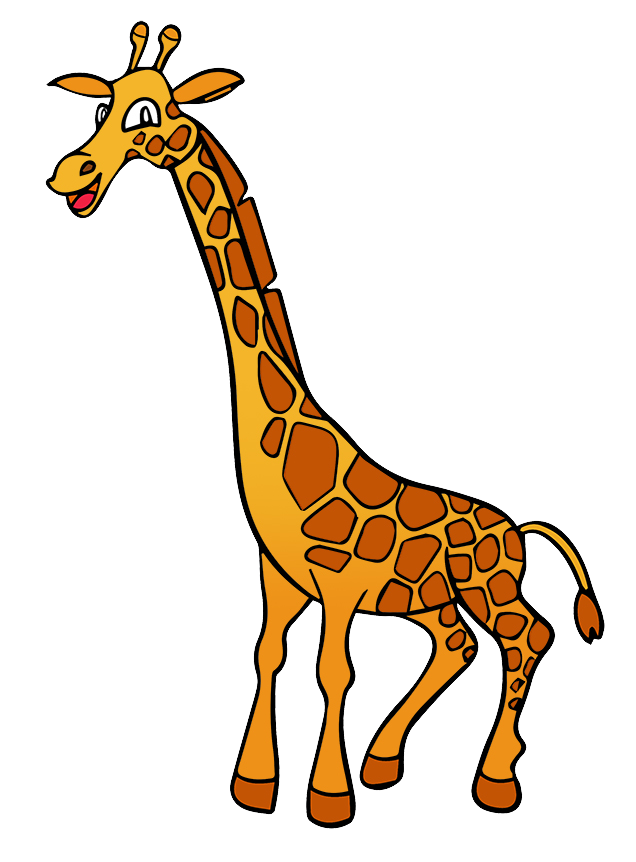
\includegraphics[width=.4\textwidth]{omnitune-client-server}
\caption{%
  High level system overview of OmniTune.%
}
\label{fig:omnitune-client-server}
\end{figure}

\subsection{Decoupling of Autotuning Service from Client Programs}

As discussed in \xref{related work}, common implementations of
autotuning in the literature either: embed the autotuning logic within
the target applications, or take a ``meta-scripting'' approach in
which the autotuner is an entirely separate program which must be
invoked by the user to tune a target application. The approach taken
in this work aims to capture the advantages of both techniques by
implementing an autotuning service with communication logic embedded
in the target applications. The resulting design consists of three
sets of components: clients, servers, and a global
database. Figure~\ref{fig:omnitune-comms} shows a typical pattern of
communication between the components.

\begin{figure}
\centering
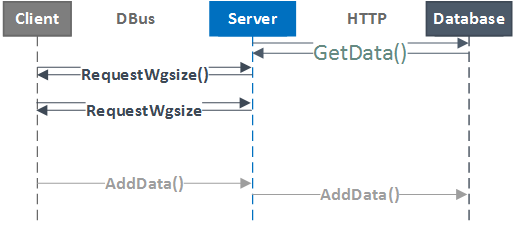
\includegraphics[width=.8\textwidth]{img/omnitune-comms}
\caption{%
  Communication pattern between OmniTune components.%
}
\label{fig:omnitune-comms}
\end{figure}

\TODO{Advantages: asynchronous communication with ``the
  cloud''. Expensive tasks such as model building aren't bound by the
  lifespan of the client application. Lightweight handling of multiple
  connections.}


\subsubsection{OmniTune Database}

A master server maintains a common store of all empirical performance
data. \TODO{Implement and write-up!}


\subsubsection{OmniTune Servers}

For each autotuning-capable machine, a system-level daemon hosts a
DBus session bus which client processes can communicate with to
request optimisation parameter values. This daemon acts as an
intermediate between the training data and the client applications. On
launch, the server requests the latest training data from the master
database, it then builds the relevant models for performing prediction
of optimisation parameter values.

OmniTune servers use a plugin system to host proxies that interface
with target applications. Proxies are application-specific, for
example, there is a proxy which implements autotuning of workgroup
size for SkelCL stencils. This proxy exposes two public methods,
\texttt{RequestWgsize} and \texttt{RequestTrainingWgsize}, shown in

Listing~\ref{lst:omnitune-proxy}.
\lstinputlisting[
  language=Python,
  float,
  floatplacement=t,
  label=lst:omnitune-proxy,
  caption={%
    Public OmniTune proxy interface for SkelCL autotuning.%
  }
]{dat/omnitune-skelcl-proxy.py}

When a SkelCL stencil is invoked, it synchronously calls the
\texttt{RequestWgsize()} method of the autotuner daemon, passing as
arguments the required data in order to assemble a feature
vector. Feature extraction then occurs within the daemon, which
classifies the datapoint and returns the suggested workgroup size to
the SkelCL process. This is a very low latency operation, and the
system daemon can handle multiple connections from separate SkelCL
processes simultaneously (although this is an admittedly unlikely
use-case given that most GPGPU programs expect to be run in
isolation).

\subsubsection{Client interface}

\lstinputlisting[
  language=C++,
  float,
  floatplacement=t,
  label=lst:skelcl-set-wgsize,
  caption={
    Implementation of SkeCL's client interface to OmniTune proxy.
  }
]{dat/skelcl-set-wgsize.cpp}

\lstinputlisting[
  language=C++,
  float,
  floatplacement=t,
  label=lst:omnitune-client,
  caption={
    Implementation of SkeCL's client interface to OmniTune proxy.
  }
]{dat/skelcl-omnitune-client.cpp}


\subsection{Distributing Training Data}


\section{Machine-learning Enabled Autotuning}


\subsection{Feature Extraction}

\TODO{The first step to developing the autotuner is feature
  extraction. That means mining the dataset to begin to correlate the
  measured dependent variable (in this case, some measure of
  performance) with explanatory variables, or features. There are
  three sets of features we are interested in: the hardware, software,
  and dataset.}

\todo{For hardware features, it's simply a case of querying the OpenCL
  API to fetch relevant device information, such as the number of
  cores available, and size of local memory. Since SkelCL supports
  multi-GPU parallelism, we'll make a note of how many devices were
  used, too.}

\todo{The software features are a little more tricky. We're looking
  for a way to capture some description of the *computation* of a
  given source code. For this, I first compile a kernel to LLVM
  bitcode, and then use the static instruction counts generated by
  LLVM's InstCount pass to generate a feature vector of the total
  instruction count and the density of different kinds of
  instructions, e.g. the number of floating point additions per
  instruction. This is sufficient for my needs but it is worth noting
  that such a crude metric may likely fall down in the presence of
  sufficiently diverging control flow, since the static instruction
  counts would no longer resemble the number of instructions actually
  executed.}

\todo{Dataset features are simple by comparison - I merely record the
  width and height of the grid, and use C++ template functions to
  stringify the input and output data types.}

For each scenario, a feature vector is extracted to capture properties
of the architecture, device, and dataset:

\begin{itemize}
\item \emph{Architectural features} --- size of local memory, maximum
  work group size, number of compute units, etc. Accessed using the
  OpenCL \texttt{clGetDeviceInfo()} API.
\item \emph{Kernel features} --- total static instruction count, ratio
  of instructions per type, ratio of basic blocks per instruction,
  etc. Accessed by compiling the OpenCL kernel to LLVM IR bitcode, and
  using the \texttt{opt} \texttt{InstCount} statistics pass.
\item \emph{Dataset features} --- size and type of the
  dataset. Accessed from the SkelCL Matrix container type.
\end{itemize}

See \FIXME{No appendix!} for a full list of features and types. For
training, feature vectors are labelled with the oracle workgroup size,
and a classifier is trained on a subset of this labelled training
data. The performance of the classifier is evaluated by comparing the
performance of the workgroup size predicted for an unseen feature
vector against the oracle workgroup size for that feature.

A full list of the feature names and types used to train machine
learning models. For training data, each feature vector was labelled
with the oracle workgroup size.

\begin{multicols}{2}
\begin{Verbatim}[fontsize=\footnotesize]
data_width                         numeric
data_height                        numeric
data_tin                           nominal
data_tout                          nominal
kern_north                         numeric
kern_south                         numeric
kern_east                          numeric
kern_west                          numeric
kern_max_wg_size                   numeric
kern_instruction_count             numeric
kern_ratio_AShr_insts              numeric
kern_ratio_Add_insts               numeric
kern_ratio_Alloca_insts            numeric
kern_ratio_And_insts               numeric
kern_ratio_Br_insts                numeric
kern_ratio_Call_insts              numeric
kern_ratio_FAdd_insts              numeric
kern_ratio_FCmp_insts              numeric
kern_ratio_FDiv_insts              numeric
kern_ratio_FMul_insts              numeric
kern_ratio_FPExt_insts             numeric
kern_ratio_FPToSI_insts            numeric
kern_ratio_FSub_insts              numeric
kern_ratio_GetElementPtr_insts     numeric
kern_ratio_ICmp_insts              numeric
kern_ratio_InsertValue_insts       numeric
kern_ratio_Load_insts              numeric
kern_ratio_Mul_insts               numeric
kern_ratio_Or_insts                numeric
kern_ratio_PHI_insts               numeric
kern_ratio_Ret_insts               numeric
kern_ratio_SDiv_insts              numeric
kern_ratio_SExt_insts              numeric
kern_ratio_SIToFP_insts            numeric
kern_ratio_SRem_insts              numeric
kern_ratio_Select_insts            numeric
kern_ratio_Shl_insts               numeric
kern_ratio_Store_insts             numeric
kern_ratio_Sub_insts               numeric
kern_ratio_Trunc_insts             numeric
kern_ratio_UDiv_insts              numeric
kern_ratio_Xor_insts               numeric
kern_ratio_ZExt_insts              numeric
kern_ratio_basic_blocks            numeric
kern_ratio_memory_instructions     numeric
kern_ratio_non_external_functions  numeric
dev_count                          numeric
dev_address_bits                   numeric
dev_double_fp_config               numeric
dev_endian_little                  numeric
dev_execution_capabilities         numeric
dev_extensions                     nominal
dev_global_mem_cache_size          numeric
dev_global_mem_cache_type          numeric
dev_global_mem_cacheline_size      numeric
dev_global_mem_size                numeric
dev_host_unified_memory            numeric
dev_image2d_max_height             numeric
dev_image2d_max_width              numeric
dev_image3d_max_depth              numeric
dev_image3d_max_height             numeric
dev_image3d_max_width              numeric
dev_image_support                  numeric
dev_local_mem_size                 numeric
dev_local_mem_type                 numeric
dev_max_clock_frequency            numeric
dev_max_compute_units              numeric
dev_max_constant_args              numeric
dev_max_constant_buffer_size       numeric
dev_max_mem_alloc_size             numeric
dev_max_parameter_size             numeric
dev_max_read_image_args            numeric
dev_max_samplers                   numeric
dev_max_work_group_size            numeric
dev_max_work_item_dimensions       numeric
dev_max_work_item_sizes_0          numeric
dev_max_work_item_sizes_1          numeric
dev_max_work_item_sizes_2          numeric
dev_max_write_image_args           numeric
dev_mem_base_addr_align            numeric
dev_min_data_type_align_size       numeric
dev_native_vector_width_char       numeric
dev_native_vector_width_double     numeric
dev_native_vector_width_float      numeric
dev_native_vector_width_half       numeric
dev_native_vector_width_int        numeric
dev_native_vector_width_long       numeric
dev_native_vector_width_short      numeric
dev_preferred_vector_width_char    numeric
dev_preferred_vector_width_double  numeric
dev_preferred_vector_width_float   numeric
dev_preferred_vector_width_half    numeric
dev_preferred_vector_width_int     numeric
dev_preferred_vector_width_long    numeric
dev_preferred_vector_width_short   numeric
dev_queue_properties               numeric
dev_single_fp_config               numeric
dev_type                           numeric
dev_vendor                         nominal
dev_vendor_id                      nominal
dev_version                        nominal
\end{Verbatim}
\end{multicols}

\subsection{Autotuning using Classification}

\TODO{Once we have features, we can create a dataset from which will
  can train a machine learning classifier. We label each feature
  vector with the size of the workgroup that gave the best
  performance.}

\todo{We now insert an autotuner into SkelCL which performs runtime
  feature extraction and classification before every stencil
  invocation.}


\subsubsection{Satisfying Constraints}

Since classifiers are probabilistic systems, it is possible that a
classifier will predict a workgroup size that is invalid for the given
scenario, $w \not\in W_{legal}(s)$. In these cases, one of three
fallback strategies is used to select a safe workgroup size:

\begin{enumerate}
\item \emph{Baseline} --- select the workgroup size which is known to be
  safe and provides the highest average case performance.
\item \emph{Random} --- select a random workgroup size uniformly from
  the set of legal values $w \in W_{legal}$.
\item \emph{Reshape} --- attempt to scale predicted the predicted
  workgroup size proportionally so that it fits within the space of
  legal workgroup sizes.
\end{enumerate}

The evaluation compares the average performance achieved using each
fallback strategy, along with the percentage of cases for which these
fallback strategies were required.

\begin{algorithm}
\begin{algorithmic}[1]
\Require kernel features $k$, hardware features $h$, dataset features
$d$.
\Ensure workgroup size $w$

\Procedure{Default}{w, a, k, d}
\Comment Use the best safe param.
\State $w \leftarrow \text{classify}(a, k, d)$
\If{$w \in W_{legal}(s)$}
    \State \textbf{return} $w$
\Else
  \State \textbf{return} $\underset{w \in W_{safe}}{\argmax}
\left(
  \prod_{s \in S_{training}} p(s, w)
\right)^{1/|S_{training}|}$
\EndIf
\EndProcedure
\item[]

\Procedure{Random}{w, a, k, d}
\Comment Use a random param from $W_{legal}$.
\State $w \leftarrow \text{classify}(a, k, d)$
\If{$w \in W_{legal}(s)$}
    \State \textbf{return} $w$
\Else
  \State \textbf{return} random choice $w \in W_{legal}$
\EndIf
\EndProcedure
\item[]

\Procedure{Reshape}{w, a, k, d}
\Comment Coerce params to be legal.
\State $w \leftarrow \text{classify}(a, k, d)$
\If{$w \in W_{legal}(s)$}
    \State \textbf{return} $w$
\Else
  \State $d_{min} \leftarrow \infty$
  \State $w_{closest} \leftarrow \text{null}$
  \For{$c \in W_{legal}$}
    \State $d \leftarrow \sqrt{\left(c_r - w_r\right)^2 + \left(c_c - w_c\right)^2}$
    \If{$d < d_{min}$}
      \State $d_{min} \leftarrow d$
      \State $w_{closest} \leftarrow c$
    \EndIf
  \EndFor
  \State \textbf{return} $w_{closest}$
\EndIf
\EndProcedure
\end{algorithmic}

\caption{Select optimal workgroup size using classification}
\label{alg:autotune-classification}
\end{algorithm}


\subsection{Autotuning using Regression}

\TODO{If we could use regression to accurately predict the runtime or
  relative performance of different workgroup sizes, then we could
  overcome the expensive training cost of autotuning by
  classification.}

% \subsubsection{Classification Using Regression}

Algorithms~\ref{alg:autotune-classification} and~\ref{alg:autotune-regression}.

\begin{algorithm}
\begin{algorithmic}[1]
\Require kernel features $k$, hardware features $h$, dataset features
$d$.
\Ensure predicted oracle workgroup size $\bar{\Omega}(s)$
\State $C \leftarrow \{c_1, c_2, \ldots, c_n \}$
\Comment Set of all workgroup sizes $\le k.\text{max\_wgsize}$
\State \textbf{return} $\underset{c \in C}{\argmin} f(k,h,d,c)$
\end{algorithmic}

\caption{Selecting workgroup size using runtime regression}
\label{alg:autotune-runtime-regression}
\end{algorithm}

\begin{algorithm}
\begin{algorithmic}[1]
\Require kernel features $k$, hardware features $h$, dataset features
$d$.
\Ensure workgroup size $w$
\State $C \leftarrow \{c_1, c_2, \ldots, c_n \}$
\Comment Set of all workgroup sizes $\le k.\text{max\_wgsize}$
\State \textbf{return} $\underset{c \in C}{\argmax} f(k,h,d,c)$
\end{algorithmic}

\caption{Selecting workgroup size using speedup regression}
\label{alg:autotune-speedup-regression}
\end{algorithm}


\subsection{Meta-tuning: a Hybrid Approach}

\begin{algorithm}
\caption{Selecting workgroup size using hybrid approach}
\label{alg:autotune-hybrid}
\begin{algorithmic}[1]
\Require kernel features $k$, hardware features $h$, dataset features $d$.
\Ensure workgroup size $c$

\State $C \leftarrow \{ c_1, c_2,\ldots, c_n \}$
\Comment Set of all workgroup sizes $\le k.\text{max\_wgsize}$

\If{no control flow in kernel}
    \State \textbf{return} $\underset{c}{\argmin} f(k,h,d,c) = r$
\Else
   \State converged $\leftarrow$ false
   \State $c_b \leftarrow$ baseline values
   \State $r_b \leftarrow$ measure runtime of runtime of program with $c_b$
   \While{not converged}
     \State return $\underset{c}{\argmax} g(k,h,d,c) = s$
     \State $r \leftarrow$ evaluate $c$
     \If{measured speedup $\frac{r_b}{r} \approx$ predicted speedup $s$}
       \State converged = true
     \Else
       \State $C = C - \{c\}$
     \EndIf
   \EndWhile
   \State \textbf{return} $c$
\EndIf
\end{algorithmic}
\end{algorithm}

\section{Summary}
